\subsection{Reproducibility of the literature search}

On June 19, 2021, we retrieved the candidate studies for the review using the
search tool available in each journal's website. This allowed us to look for
the instances in which the 'natural experiment*' token 
Table \ref{tab:journal_search}
reports the set of urls we visited. For the journals published by 'John Wiley \&
Sons' we were not allowed to compose our search query using the wild-car symbol '*.'
Therefore, to ensure the commensurability of results across journals, we
run two separate queries, namely, `natural experiment' and `natural
experiment\textbf{s}.'

\begin{table*}
  \centering
  \sffamily
  \begin{small}
    \resizebox{1\textwidth}{!}{%
\begin{tabular}[c]{ll}
  \toprule \toprule
  \multicolumn{1}{l}{Journal} & 
  \multicolumn{1}{l}{Address of the search page} \\
  \midrule
  Academy Of Management Journal\dotfill & \url{https://journals.aom.org/search/advanced}\\
  Administrative Science Quarterly\dotfill & \url{https://journals.sagepub.com/search/advanced?SeriesKey=asqa}\\             
  Entrepreneurship Theory \& Practice\dotfill & \url{https://journals.sagepub.com/search/advanced?SeriesKey=etpb}\\         
  Journal of Business Ethics\dotfill & \url{https://link.springer.com/search?query=&search-within=Journal&facet-journal-id=10551}\\                 
  Journal of Business Venturing\dotfill & \url{https://www.sciencedirect.com/journal/journal-of-business-venturing}\\                
  Journal of Management\dotfill & \url{https://journals.sagepub.com/search/advanced?SeriesKey=joma}\\                        
  Journal of Management Studies\dotfill & \url{https://onlinelibrary.wiley.com/search/advanced?publication=14676486&text1=}\\                
  Management Science\dotfill & \url{https://pubsonline.informs.org/action/doSearch?SeriesKey=mnsc}\\                           
  Organization Science\dotfill & \url{https://pubsonline.informs.org/action/doSearch?SeriesKey=orsc}\\                         
  Organization Studies\dotfill & \url{https://journals.sagepub.com/search/advanced?SeriesKey=oss}\\                        
  Research Policy\dotfill & \url{https://www.sciencedirect.com/journal/research-policy}\\                              
  Strategic Entrepreneurship Journal\dotfill & \url{https://onlinelibrary.wiley.com/search/advanced?publication=1932443x&text1=}\\           
  Strategic Management Journal\dotfill & \url{https://onlinelibrary.wiley.com/search/advanced?publication=10970266&text1=}\\
  Strategic Organization\dotfill & \url{https://journals.sagepub.com/search/advanced?SeriesKey=soq}\\                        
  The Leadership Quarterly\dotfill & \url{https://www.sciencedirect.com/journal/the-leadership-quarterly}\\                         
  \bottomrule
\end{tabular}
}
  \end{small}
  \label{tab:journal_search}
  \caption{Sample of target journals along with search page addresses.}
\end{table*}

\subsection{Sampling}

To consistently sample the studies for the review, two co-authors independently 
went through a random sample of twenty items and created a tentative set of
exclusion categories. Then, the whole team of co-authors collectively evaluated
the codes included in each set of exclusion categories, normalized the codes,
and created the sampling worflow portrayed in Figure \ref{fig:sampling_workflow}.

\begin{figure*}
	\begin{small}
		\begin{center}
			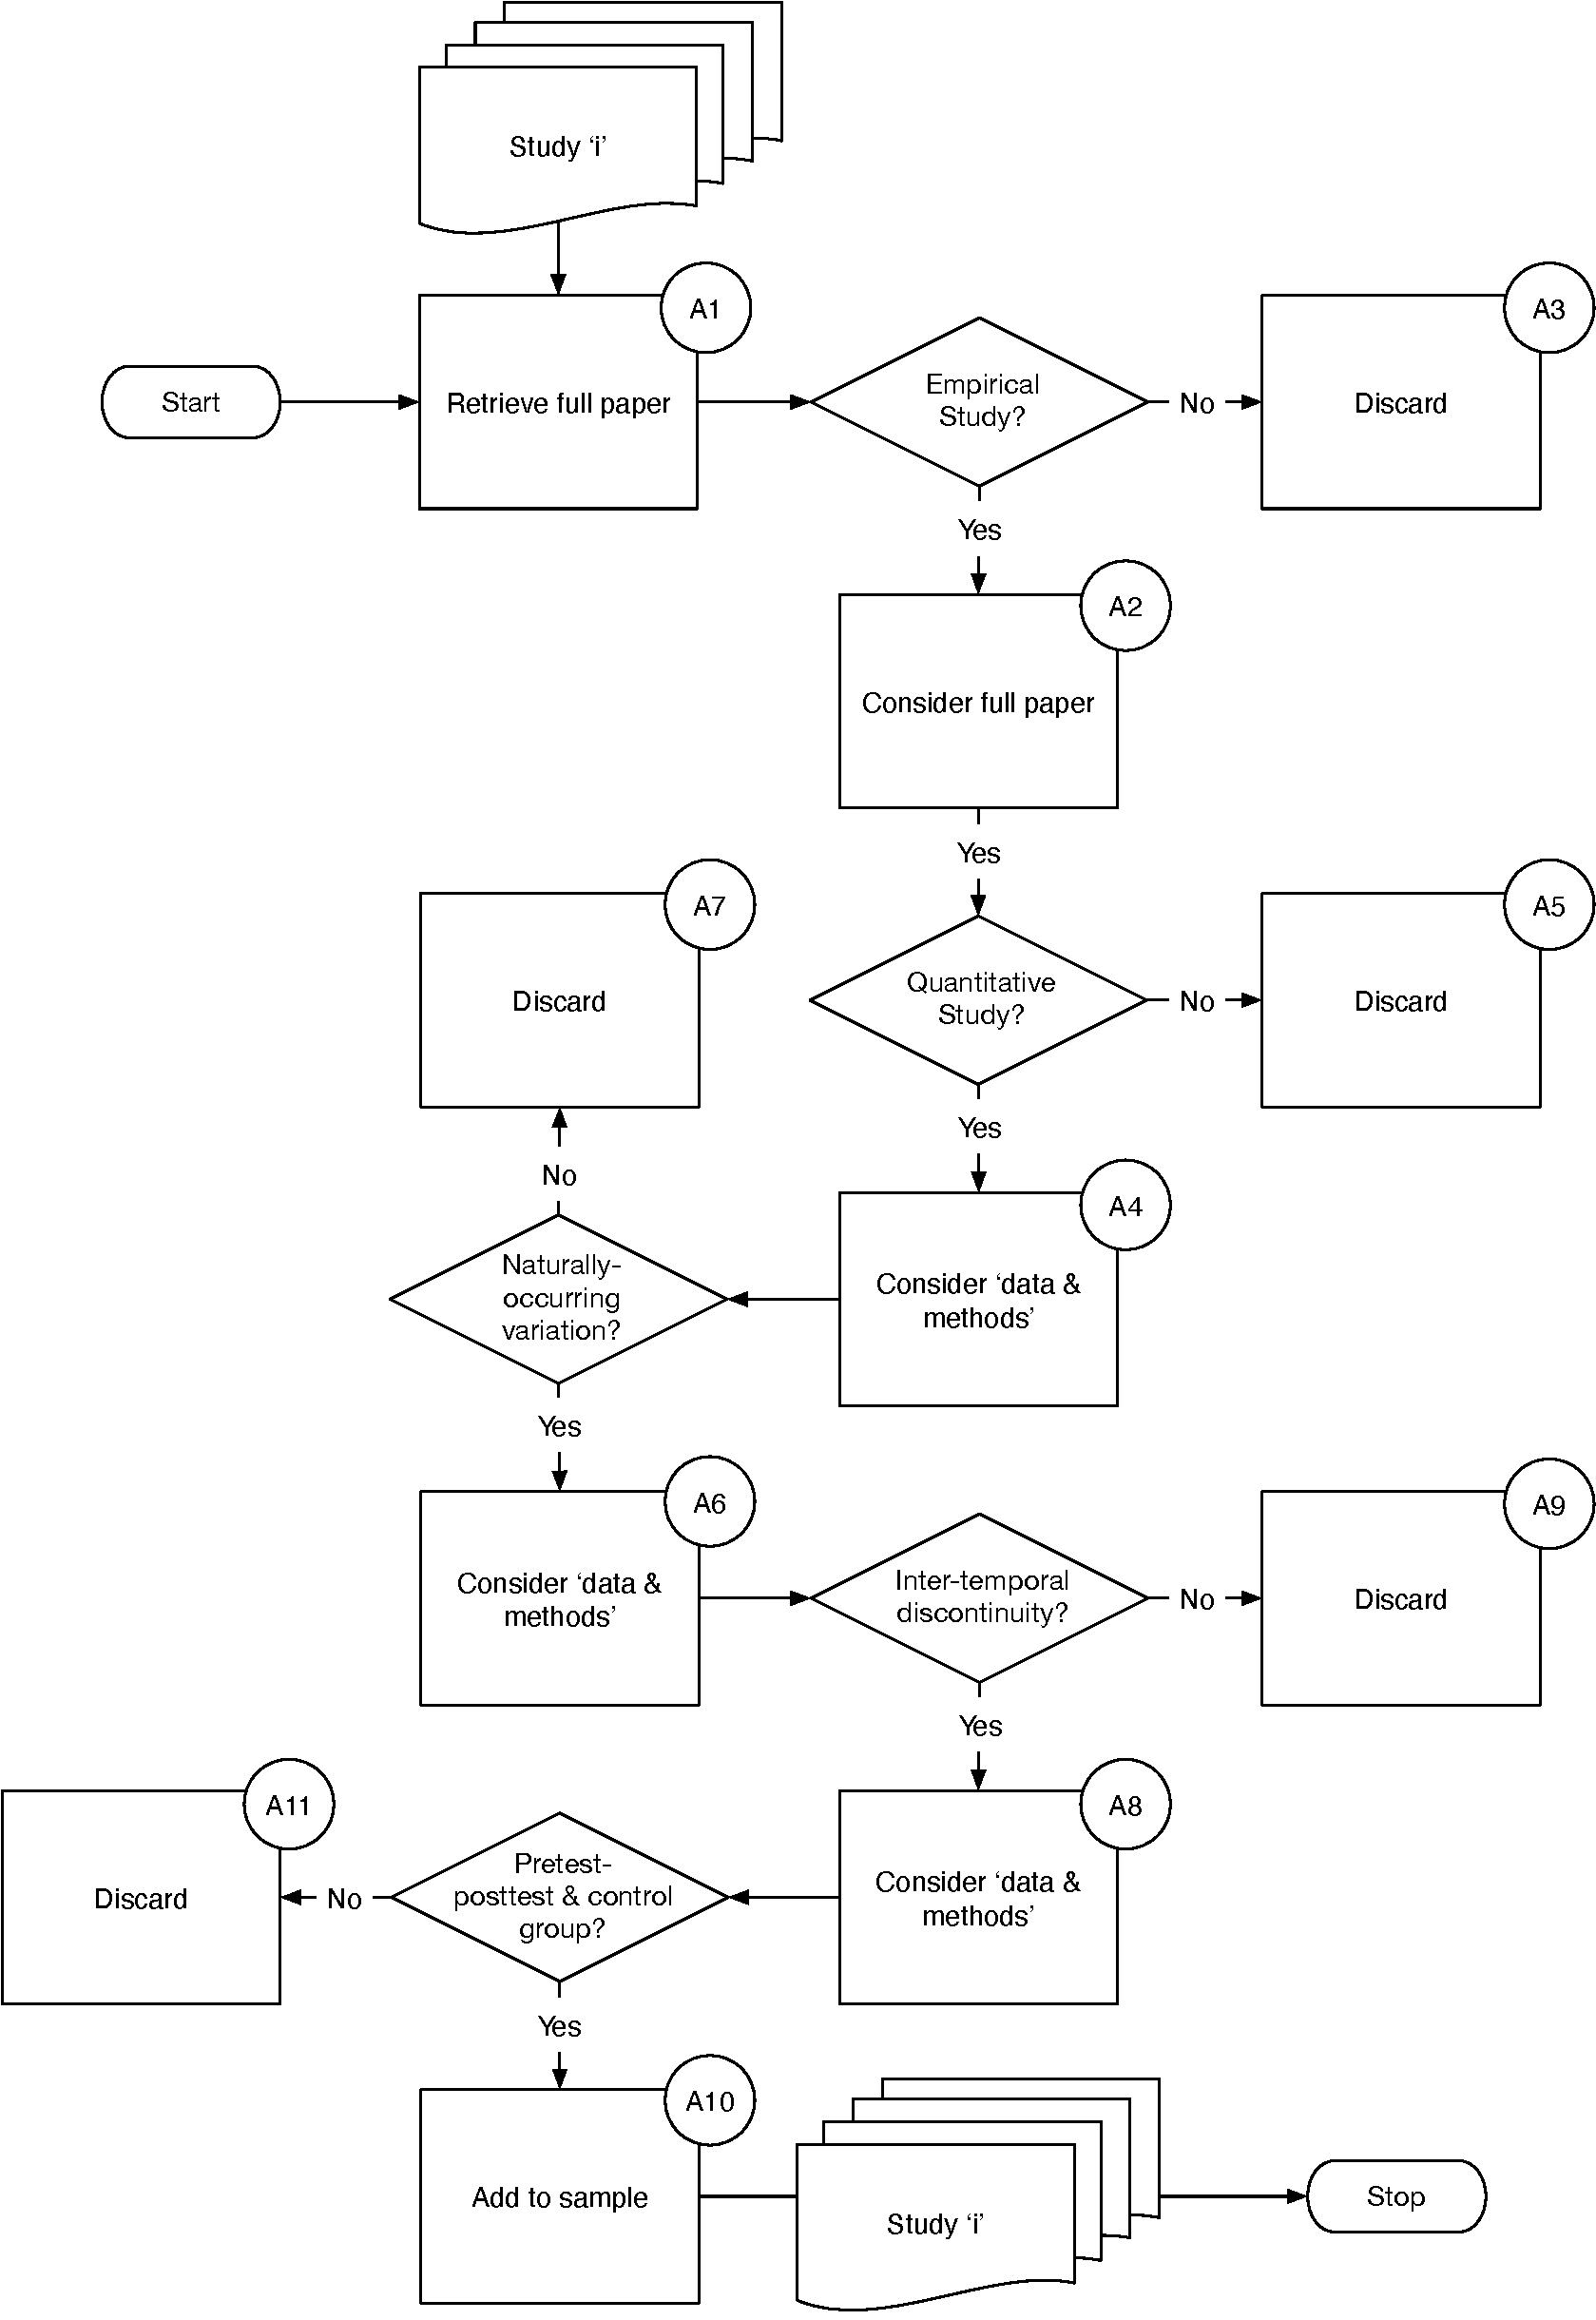
\includegraphics[width=0.95\textwidth]{exhibits/sampling_workflow.pdf}
		\end{center}
		\caption{Sampling workflow}
		\label{fig:sampling_workflow}
	\end{small}
\end{figure*}

First, we removed non-empirical works, such as conceptual studies 
\parencite[e.g.,][]{eden2021}, literature reviews
\parencite[e.g.,][]{shaver2020}, meta-analysis
\parencite[e.g.,][]{geyskens2006}, calls for papers
\parencite[e.g.,][]{jacquart2020}, or editorial notes
\parencite[e.g.,][]{breschi2020}. With few exceptions
\parencite[e.g.,][]{sieweke2020}, the NE design plays a peripheral role in this
category's studies. Second, we removed ten qualitative empirical works that 
denote the empirical setting as a 'natural experiment' \parencite[][]{} or that mirror
the logic of a natural experiments \parencite[e.g.,][]{powell2017}, a case study
design that Eisenhardt recently labeled ``racing design'' since \textit{``cases
(often ventures) begin at the same time with similar initial conditions like
founders, location, and funding, and then `race' to some natural endpoint like
IPO, unicorn valuation, or other temporal marker.''} \parencite[page
150,][]{eisenhardt2021}.  Third, we removed quantitative empirical works that limit to refer
to previous natural experiment studies \parencite[e.g.,][]{stevens2021}, discuss
a project's limitations in regard to the lack of a natural experiment
\parencite[e.g.,][]{chen2020}, or indicate natural experiments as a future
research avenues \parencite[e.g.,][]{xie0000}.  Fourth, we removed empirical
works that claim to use a natural experiment whereas they do not exploit any
sudden naturally occurring, sudden variations in the data. Such a category
includes studies that --- in fact --- use field experiments
\parencite[e.g.,][]{lee2017}, quasi-experiments
\parencite[e.g.,][]{azoulay2014}, laboratory/online experiments
\parencite[e.g.,][]{laurieromartinez2014}, twin research design
\parencite[e.g.,][]{nicolaou2008}, or correlational research designs
\parencite[e.g.,][]{boyle2011}. Fifth, we removed empirical works that exploit a
naturally occurring variation to operate the instrumental variable
\parencite[e.g.,][]{zolotoy2018} or the regression discontinuity research design
\parencite[e.g.,][]{flammer2015}.  Finally, we removed empirical works that
exploit a sudden, naturally-occurring  variation but lack either a comparison
group \parencite[e.g.][]{corbo2016} or pre-treatment data
\parencite[e.g.,][]{desjardine2019}.

\ref{fig:exclusion_causes}. 

\begin{figure*}
    \centering
    \sffamily
    \begin{small}
        \begin{center}
            \begin{tikzpicture}
    \begin{axis}[
      width=6cm, height=8cm,
      mark size=2pt,
      xlabel={Counts of excluded studies},
      %ylabel={Counts of studies},
      ytick={1,2,3,4,5,6,7,8,9},
      yticklabels={
        Correlational studies,
        Field experiment studies,
        Laboratory experiment studies,
		    Quasi-experimental studies, 
        Twin research design studies,
        Instrumental variable studies,
		    Regression discontinuity design studies,
        One-group pretest-posttest studies (interrupted time series),
        Posttest-only studies with (nonequivalent) control groups,
        %Standard NE studies,
        },
      axis y line*=left,
      axis x line*=bottom,
      axis line style={draw=none},
      nodes near coords,
      nodes near coords align={horizontal},
      every node near coord/.append style={inner sep=4pt},
      point meta=rawx
    ]
    \addplot + [xcomb] [
        black, mark options={black}
    ] table {exhibits/exclusion_categories.dat};
  \end{axis}
\end{tikzpicture}       
        \end{center}
        \caption{Distribution of the retrieved studies across exclusion 
        categories.}
        \label{fig:exclusion_causes}
    \end{small}
\end{figure*}
